\section{Vehicle}
The rover uses an Ackermann steering mechanism to be able to navigate, like that seen in Figure~\ref{sample_return_rover:fwd_kin:ackermann}. Unlike the average robotic arm, it is not a serial connection. Forward kinematics cannot be used on a mobile robot. Ackermann steering allows the front wheels to rotate independently, about a common center point. This center point is called the \textit{Instantaneous Center of Curvature} (ICC). In general, it uses a four bar linkage in a trapezoidal shape. However the Curiosity Mars Rover and the Sample-Return Rover does not use this linkage, but the model still holds.

\begin{figure}[H]
	\centering
	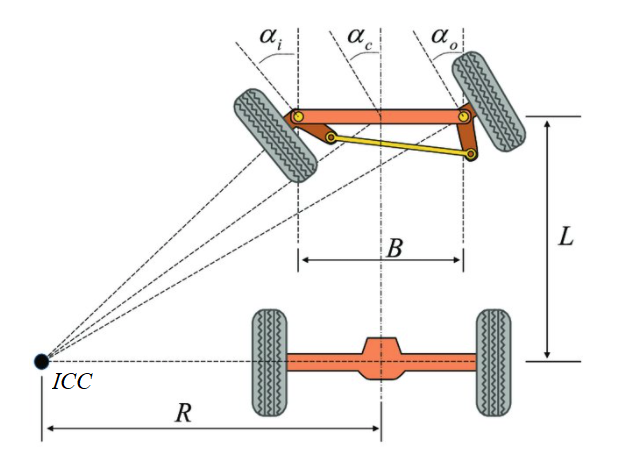
\includegraphics[scale=0.65]{sections/robot-design/images/ackermann_steering.png}
	\caption{Diagram for Ackermann Steering}
	\label{sample_return_rover:fwd_kin:ackermann}
\end{figure}

\section{Arm}
In robotics, forward kinematics is used to find the position and orientation of the robot's end-effector (or gripper) given the joint angles. In this course, joints can have two different types: \textit{revolute} and \textit{prismatic}. A revolute joint rotates about an axis, while a prismatic joint translates linearly along an axis. In serial kinematic chains, such as the arm seen in Figure~\ref{sample_return_rover:robot_design:arm_side}, each coordinate frame assigned to the distal end of a link \textit{i} is dependent on the position and geometry of the $(i-1)^{th}$ joint and link, respectively. The frame \textit{i} resolved in frame \textit{i - 1} represents a combination of a rotation performed by the $(i-1)^{th}$ joint with a successive translation down the length of link \textit{i - 1}. Chaining these homogeneous transformation matrices together results in the transformation of the end-effector in the robot's base frame. \\

The robot arm itself is \ac{4DOF} where each joint is revolute. However, as seen in Figure~\ref{sample_return_rover:robot_design:arm_frames}, there are eight frames in total, because four dummy frames are for Gazebo to properly render in the arm. Its corresponding DH table is shown in Table~\ref{sample_return_rover:robot_design:dh}, and the values for the nonzero static lengths can be seen in Table~\ref{sample_return_rover:robot_design:dh_values}. A list of the links are shown in Figure~\ref{sample_return_rover:robot_design:arm_diagram}. The links \textit{LeftFinger} and \textit{RightFinger} are just there for Gazebo to be able to rotate the end-effector fingers, but they are not used in the DH parameters and table. \\

Note that the arm's home position starts with all angles being at 0, so the arm is fully upward. Each joint has a limit for its range of motion so that the robot does not crash into itself. Equation~\ref{sample_return_rover:robot_design:th1} to \ref{sample_return_rover:robot_design:th4} offer reasonable ranges of allowable motion.

\begin{figure}[htbp]
	\centering
	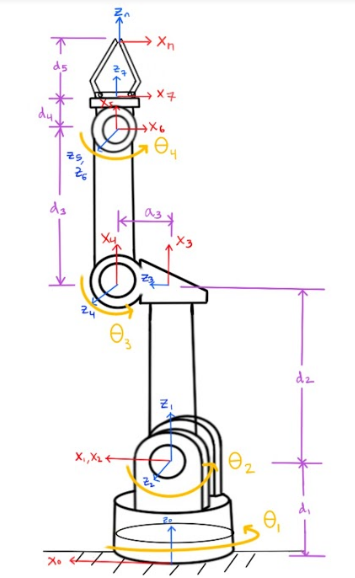
\includegraphics[scale=0.6]{sections/robot-design/images/arm_frames.png}
	\label{sample_return_rover:robot_design:arm_frames}
	\caption{DH Frames of the Arm}
\end{figure}

\begin{figure}[H]
	\centering
	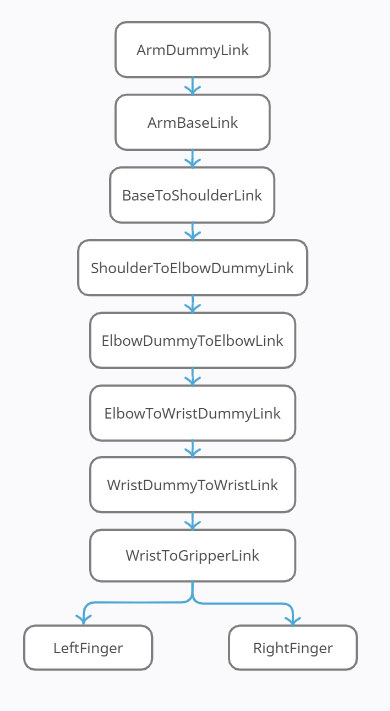
\includegraphics[scale=0.75]{sections/robot-design/images/arm_link_diagram.png}
	\label{sample_return_rover:robot_design:arm_diagram}
	\caption{Flowchart of the Arm Links}
\end{figure}

\begin{table}[htbp]
	\centering
	\begin{tabular}{|c|c|c|c|c|}
		\hline
		\textit{Link i} & \textit{$\theta$} & \textit{d} & \textit{$\alpha$} & \textit{a}\\
		\hline
		1 & $\theta_{1}$ & $d_{1}$ & 0 & 0 \\
		2 & 0 & 0 & -90 & 0 \\
		3 & $\theta_{2}$ - 90  & 0 & -90 & $d_{2}$ \\
		4 & 0  & $a_{3}$ & 90 & 0 \\
		5 & $\theta_{3}$ & 0 & 0 & $d_{3}$ \\
		6 & $\theta_{4}$ - 90 & 0 & -90 & 0 \\
		7 & 0 & $d_{4}$ & 0 & 0 \\
		n & 0 & $d_{5}$ & 0 & 0 \\
		\hline
	\end{tabular}
	\label{sample_return_rover:robot_design:dh}
	\caption{DH Table for the Arm}
\end{table}

\begin{table}[H]
	\centering
	\begin{tabular}{|c|c|}
		\hline
		\textit{Distance between Frames} & \textit{Length} \\
		\hline
		Base to Frame 1 ($d_{1}$) & 2.9in \\
		Frame 2 to Frame 3 ($d_{2}$) & 7.73in \\
		Frame 3 to Frame 4 ($a_{3}$) & 1.76in \\
		Frame 4 to Frame 5 ($d_{3}$) & 8.93in \\
		Frame 6 to Frame 7 ($d_{4}$) & 1in \\
		Frame 7 to Frame n ($d_{5}$) & 1.41in \\
		\hline
	\end{tabular}
	\label{sample_return_rover:robot_design:dh_values}
	\caption{Table of Link Lengths of the Arm}
\end{table}

\begin{equation}\label{sample_return_rover:robot_design:th1}
	\theta_{1} = [-\pi,\; + \pi]
\end{equation}

\begin{equation}\label{sample_return_rover:robot_design:th2}
	\theta_{2} = \left[0,\; +\frac{2\pi}{3}\right]
\end{equation}

\begin{equation}\label{sample_return_rover:robot_design:th3}
	\theta_{3} = [0,\; + \pi]
\end{equation}	

\begin{equation}\label{sample_return_rover:robot_design:th4}
	\theta_{4} = \left[-\frac{2\pi}{3},\; +\frac{2\pi}{3}\right]
\end{equation} \\

One method to start calculating the forward kinematics is to create DH matrices $T^{n-1}_{n}$, which are composed of rotations about the z-axis, translations in the z-axis, rotations about the x-axis, and finally translations in the x-axis. The basic rotation matrix for a rotation about the z-axis with an angle $\theta$ can be shown in Equation~\ref{sample_return_rover:robot_design:rz}, and Equation~\ref{sample_return_rover:robot_design:rx} for rotation about the x-axis by angle $\alpha$. The translation vectors can be seen in Equations~\ref{sample_return_rover:robot_design:dx} and~\ref{sample_return_rover:robot_design:dz} for along the z and x axes by a displacement \textit{d} and \textit{a}, respectively. Using the DH Table, the homogeneous transformation matrices can now be written. The setup for this matrix is seen in Equation~\ref{sample_return_rover:robot_design:H0n}.

\begin{equation}
	R_{z, \theta} = \left[\begin{array}{ccc}
		cos(\theta) & sin(\theta) & 0 \\
		sin(\theta) & cos(\theta) & 0 \\
		0 & 0 & 1
	\end{array}\right]
\label{sample_return_rover:robot_design:rz}
\end{equation}

\begin{equation}
	R_{x, \alpha} = \left[\begin{array}{ccc}
		1 & 0 & 0 \\
		0 & cos(\alpha) & -sin(\alpha) \\
		0 & sin(\alpha) &  cos(\alpha) \\
		\end{array}\right]
	\label{sample_return_rover:robot_design:rx}
\end{equation}

\begin{equation}
	t^{n-1}_{n_{z}} = \left[\begin{array}{c}
		0 \\
		0 \\
		d
	\end{array}\right]
	\label{sample_return_rover:robot_design:dz}
\end{equation}

\begin{equation}
	t^{n-1}_{n_{x}} = \left[\begin{array}{c}
		a \\
		0 \\
		0
	\end{array}\right]
	\label{sample_return_rover:robot_design:dx}
\end{equation}

\begin{equation}
	H^{0}_{n} = \left[\begin{array}{cc}
		R^{0}_{n} & t^{0}_{n} \\
	    0 & 1
	\end{array}\right]
\label{sample_return_rover:robot_design:H0n}
\end{equation} \\

Another method is to observe the geometry of the workspace, which is the set of positions and orientations that the end effector can accomplish, and find the restrictions created by it. This type of approach was taken for this project to solve for the four dimensions of actuation, the 3D position $\left[x^{0}_{n} \; y^{0}_{n}\; z^{0}_{n}\right]^{T}$ and a rotation off the z-axis of the robot's shoulder joint $\gamma$. \\

The base joint is the only one that rotates about the base's z-axis, so the values for $x^{0}_{n}$ and $y^{0}_{n}$ can be thought of as a projection of the arm on to the ($x_{0}$,$y_{0}$) plane, where the length of this projection is a function of the shoulder, elbow, and wrist joints, as well as their child links. This length rotates about the z axis with the base joint. This geometry describes how to derive $x^{0}_{n}$ and $y^{0}_{n}$, seen in Equations~\ref{sample_return_rover:fwd_kinematics:x0n} and~\ref{sample_return_rover:fwd_kinematics:y0n}. The z coordinate by definition is the displacement of linkage in the z-axis. Considering the fact that the rest of the three joints act in the xz plane, the solution can be solved as a summation of the length of each link that traverses its local x-axis times the cosine of the net angle and the length of each link that traverses its local z-axis times the sine of the net angle. For this arm, that results in Equation~\ref{sample_return_rover:fwd_kinematics:z0n}, as $\theta_{1}$ can not cause actuation in the z-axis. Finally, because $\gamma$ is essentially the angle between the xy plane of the base and the surface that the vehicle is on, assuming that the vehicle is flat relative to the surface, then $\gamma$ can be solved with Equation~\ref{sample_return_rover:fwd_kinematics:gamma}.

\begin{equation}\label{sample_return_rover:fwd_kinematics:x0n}
	x^{0}_{n} = c_{1}\left(d_{2}s_{2}+a_{2}c_{2}+d_{3}s_{23}+(d_{4}+d_{5})s_{234}\right)
\end{equation}

\begin{equation}\label{sample_return_rover:fwd_kinematics:y0n}
	y^{0}_{n} = s_{1}\left(d_{2}s_{2}+a_{2}c_{2}+d_{3}s_{23}+(d_{4}+d_{5})s_{234}\right)
\end{equation}

\begin{equation}\label{sample_return_rover:fwd_kinematics:z0n}
	z^{0}_{n} = d_{1}+d_{2}c_{2}-a_{2}s_{2}+d_{3}c_{23}+(d_{4}+d_{5})c_{234}
\end{equation}

\begin{equation}\label{sample_return_rover:fwd_kinematics:gamma}
	\gamma = \theta_{2} + \theta_{3} + \theta_{4}
\end{equation}

Where:

\begin{equation}\label{sample_return_rover:fwd_kinematics:cij}
	c_{ij...} = cos(\theta_{i} + \theta_{j} + ...)
\end{equation}

\begin{equation}\label{sample_return_rover:fwd_kinematics:sij}
	s_{ij...} = sin(\theta_{i} + \theta_{j} + ...)
\end{equation}
